\documentclass{beamer}
\mode<presentation>
\usepackage{amsmath}
\usepackage{amssymb}
%\usepackage{advdate}
\usepackage{adjustbox}
\usepackage{subcaption}
\usepackage{enumitem}
\usepackage{multicol}
\usepackage{mathtools}
\usepackage{listings}
\usepackage{physics}
\usepackage{url}
\def\UrlBreaks{\do\/\do-}
\usetheme{Boadilla}
\usecolortheme{lily}
\setbeamertemplate{footline}
{
  \leavevmode%
  \hbox{%
  \begin{beamercolorbox}[wd=\paperwidth,ht=2.25ex,dp=1ex,right]{author in head/foot}%
    \insertframenumber{} / \inserttotalframenumber\hspace*{2ex} 
  \end{beamercolorbox}}%
  \vskip0pt%
}

\providecommand{\nCr}[2]{\,^{#1}C_{#2}} % nCr
\providecommand{\nPr}[2]{\,^{#1}P_{#2}} % nPr
\providecommand{\mbf}{\mathbf}
\providecommand{\pr}[1]{\ensuremath{\Pr\left(#1\right)}}
\providecommand{\qfunc}[1]{\ensuremath{Q\left(#1\right)}}
\providecommand{\sbrak}[1]{\ensuremath{{}\left[#1\right]}}
\providecommand{\lsbrak}[1]{\ensuremath{{}\left[#1\right.}}
\providecommand{\rsbrak}[1]{\ensuremath{{}\left.#1\right]}}
\providecommand{\brak}[1]{\ensuremath{\left(#1\right)}}
\providecommand{\lbrak}[1]{\ensuremath{\left(#1\right.}}
\providecommand{\rbrak}[1]{\ensuremath{\left.#1\right)}}
\providecommand{\cbrak}[1]{\ensuremath{\left\{#1\right\}}}
\providecommand{\lcbrak}[1]{\ensuremath{\left\{#1\right.}}
\providecommand{\rcbrak}[1]{\ensuremath{\left.#1\right\}}}
\theoremstyle{remark}
\newtheorem{rem}{Remark}
\newcommand{\sgn}{\mathop{\mathrm{sgn}}}
\providecommand{\abs}[1]{\left\vert#1\right\vert}
\providecommand{\res}[1]{\Res\displaylimits_{#1}} 
\providecommand{\norm}[1]{\lVert#1\rVert}
\providecommand{\mtx}[1]{\mathbf{#1}}
\providecommand{\mean}[1]{E\left[ #1 \right]}
\providecommand{\fourier}{\overset{\mathcal{F}}{ \rightleftharpoons}}
%\providecommand{\hilbert}{\overset{\mathcal{H}}{ \rightleftharpoons}}
\providecommand{\system}{\overset{\mathcal{H}}{ \longleftrightarrow}}
	%\newcommand{\solution}[2]{\textbf{Solution:}{#1}}
%\newcommand{\solution}{\noindent \textbf{Solution: }}
\providecommand{\dec}[2]{\ensuremath{\overset{#1}{\underset{#2}{\gtrless}}}}
\newcommand{\myvec}[1]{\ensuremath{\begin{pmatrix}#1\end{pmatrix}}}
\let\vec\mathbf

\lstset{
%language=C,
frame=single, 
breaklines=true,
columns=fullflexible
}

\numberwithin{equation}{section}

\lstset{
  language=Python,
  basicstyle=\ttfamily\small,
  keywordstyle=\color{blue},
  stringstyle=\color{orange},
  numbers=left,
  numberstyle=\tiny\color{gray},
  breaklines=true,
  showstringspaces=false
}

\title{Problem 2.8.2}
\author{ee25btech11023-Venkata Sai}

\date{\today} 
\begin{document}

\begin{frame}
\titlepage
\end{frame}

\section*{Outline}
\begin{frame}
\tableofcontents
\end{frame}
\section{Problem}
\begin{frame}
\frametitle{Problem Statement}
%
$\vec{A}\brak{6,1},\vec{B}\brak{8, 2}$ and $\vec{C}\brak{9, 4}$ are three vertices of a parallelogram $ABCD$. If $E$ is the
midpoint of DC find the area of $\triangle$ADE. 
\end{frame}
%\subsection{Literature}
\section{Solution}
\subsection{Formula}
\begin{frame}
\frametitle{Formula}
\setcounter{section}{1}
%\framesubtitle{Literature}
To Find Area of Triangle
\begin{align}
\text{Area\brak{\triangle ADE}}&=\frac12\norm{\brak{\vec{D}-\vec{A}}\times\brak{\vec{E}-\vec{A}}}
\end{align}

\end{frame}
\subsection{Finding the Point D}
\begin{frame}
\frametitle{Finding the Point D}

\begin{align}
\vec{B}&-\vec{A}=\vec{C}-\vec{D} \\
    \vec{D}&=\vec{C}+\vec{A}-\vec{B} \\
    \vec{D}&=\myvec{9\\4}+\myvec{6\\1}-\myvec{8\\2} \\
    \vec{D}&=\myvec{7\\3}
\end{align}
\end{frame}
\subsection{Finding the midpoint of DC and Area($\triangle$ADE)}
\begin{frame}
\frametitle{Finding the midpoint of DC and Area($\triangle$ADE)}
\begin{align}
\vec{E}=\frac{\vec{D}+\vec{C}}2 =\frac{\myvec{7\\3}+\myvec{9\\4}}2=\myvec{8\\\frac{7}2} 
\end{align}
\begin{align}
\vec{D}-\vec{A}=\myvec{7\\3}-\myvec{6\\1}=\myvec{1\\2},\vec{E}-\vec{A}=\myvec{8\\\frac72}-\myvec{6\\1}=\myvec{2\\\frac52} 
\end{align}
\end{frame}

\subsection{Area($\triangle$ADE)}
\begin{frame}
\frametitle{Area($\triangle$ADE)}
\begin{align}
\text{Area\brak{\triangle ADE}}&=\frac12\norm{\brak{\vec{D}-\vec{A}}\times\brak{\vec{E}-\vec{A}}} \\
& =\frac12\norm{\myvec{1\\2}\times \myvec{2\\\frac52}} = \frac{1}{2}\mdet{1 & 2 \\ 2 & \frac{5}{2}}=\frac{3}{4} 
\end{align}
Hence the Area of triangle is $\frac{3}{4}$ units.
\end{frame}

\subsection{Plot}
\begin{frame}[fragile]
\frametitle{Plot}

\begin{figure}[h!]
   \centering
   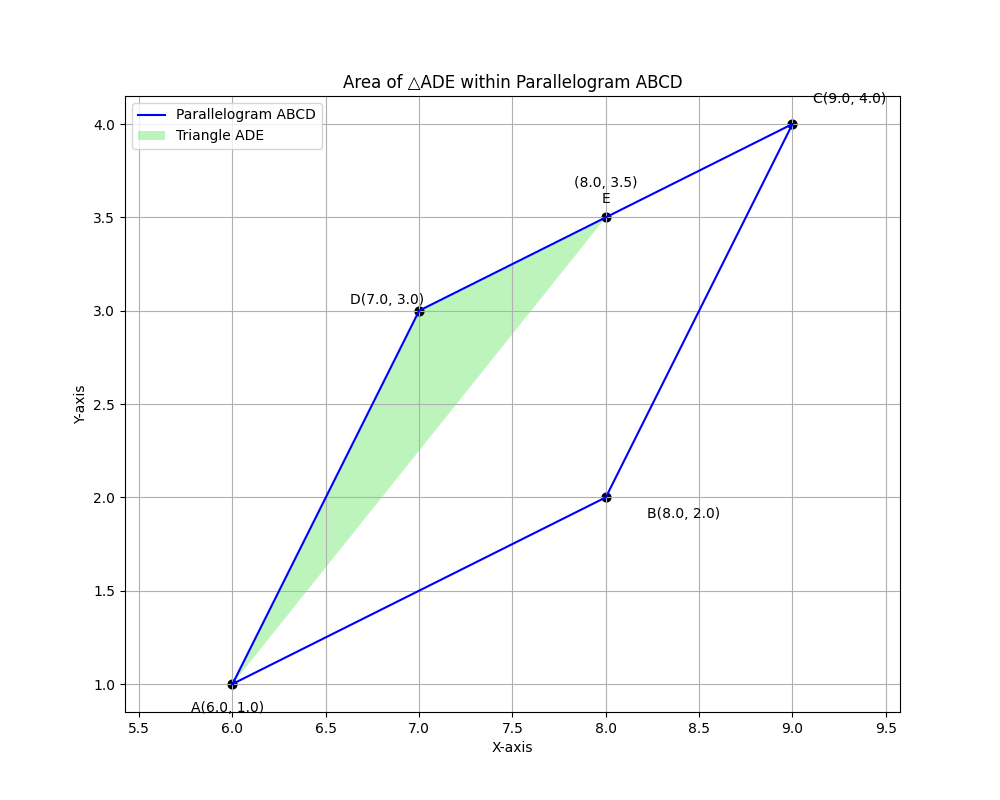
\includegraphics[width=0.7\columnwidth]{figs/fig1.png}
	\caption{}
   \label{stemplot}
\end{figure}
\end{frame}

\section{C Code}
\begin{frame}[fragile]
\frametitle{C Code for finding points}
\begin{lstlisting}[language=C]
void calculate_parallelogram_coords(double* out_coords) {
    // Given vertices
    double Ax = 6.0, Ay = 1.0;
    double Bx = 8.0, By = 2.0;
    double Cx = 9.0, Cy = 4.0;
    
    double Dx = Ax - Bx + Cx;
    double Dy = Ay - By + Cy;

    double Ex = (Dx + Cx) / 2.0;
    double Ey = (Dy + Cy) / 2.0;
  
    out_coords[0] = Ax; out_coords[1] = Ay;
    out_coords[2] = Bx; out_coords[3] = By;
    out_coords[4] = Cx; out_coords[5] = Cy;
    out_coords[6] = Dx; out_coords[7] = Dy;
    out_coords[8] = Ex; out_coords[9] = Ey;
}
    \end{lstlisting}
\end{frame}
\section{Python Code}
\begin{frame}[fragile]
\frametitle{Calling C Function}
\begin{lstlisting}[language=Python]
import ctypes
import numpy as np

def get_all_points():
  
    # Load the compiled C shared library
    lib = ctypes.CDLL('./coord.so')
    lib.calculate_parallelogram_coords.argtypes = [ctypes.POINTER(ctypes.c_double)]

    out_coords_c = double_array_10()

    # Call the C function, passing the C array by reference
    lib.calculate_parallelogram_coords(out_coords_c)

    # Convert the C array result back into a NumPy array
    # Reshape it to 5x2 (5 points, each with x and y)
    all_points = np.array(out_coords_c).reshape(5, 2)
    return all_points
\end{lstlisting}
\end{frame}

\begin{frame}[fragile]
\frametitle{Python Code for Plotting}
\begin{lstlisting}[language=Python]
#Code by GVV Sharma
#September 12, 2023
#Revised July 21, 2024
#released under GNU GPL

import sys
import numpy as np
import matplotlib.pyplot as plt
sys.path.insert(0, '/workspaces/urban-potato/matgeo/codes/CoordGeo/') 
# --- Import from our C Interface Module ---
from call import get_all_points

from line.funcs import *
from triangle.funcs import *
from conics.funcs import circ_gen

\end{lstlisting}
\end{frame}

\begin{frame}[fragile]
\frametitle{Python Code for Plotting}
\begin{lstlisting}[language=Python]
points=get_all_points()
A, B, C, D, E = points

print(f"Midpoint E coordinates: ({E[0]:.1f}, {E[1]:.1f})")
# Calculate and print the area of triangle ADE
area_ADE = 0.5 * np.abs(A[0]*(D[1] - E[1]) + D[0]*(E[1] - A[1]) + E[0]*(A[1] - D[1]))
print(f"The area of Triangle ADE is: {area_ADE}")

# --- Plotting ---
fig, ax = plt.subplots(figsize=(10, 8))

# Draw and fill the shapes
ax.plot(np.vstack([A, B, C, D, A])[:, 0], np.vstack([A, B, C, D, A])[:, 1], 'b-', label='Parallelogram ABCD')
ax.fill(np.vstack([A, D, E, A])[:, 0], np.vstack([A, D, E, A])[:, 1], 'lightgreen', alpha=0.6, label='Triangle ADE')
\end{lstlisting}
\end{frame}

\begin{frame}[fragile]
\frametitle{Python Code for Plotting}
\begin{lstlisting}[language=Python]
# Draw the vertices
ax.scatter(points[:, 0], points[:, 1], color='black', s=40)

# Add annotations with specific offsets
ax.annotate(f'A({A[0]:.1f}, {A[1]:.1f})', xy=A, xytext=(-30, -20), textcoords='offset points')
ax.annotate(f'B({B[0]:.1f}, {B[1]:.1f})', xy=B, xytext=(30, -15), textcoords='offset points')
ax.annotate(f'C({C[0]:.1f}, {C[1]:.1f})', xy=C, xytext=(15, 15), textcoords='offset points')
ax.annotate(f'D({D[0]:.1f}, {D[1]:.1f})', xy=D, xytext=(-50, 5), textcoords='offset points')
ax.annotate(f'({E[0]:.1f}, {E[1]:.1f})\nE', xy=E, xytext=(0, 8), textcoords='offset points', ha='center', va='bottom')
\end{lstlisting}
\end{frame}

\begin{frame}[fragile]
\frametitle{Python Code for Plotting}
\begin{lstlisting}[language=Python]
# --- Final Formatting ---
ax.set_xlabel('X-axis')
ax.set_ylabel('Y-axis')
ax.set_title('Area of Triangle ADE within Parallelogram ABCD')
ax.grid(True)
ax.axis('equal')
ax.legend()
plt.show()
plt.savefig('../figs/fig1.png')
\end{lstlisting}
\end{frame}

\end{document}
